\documentclass[a4paper, 12pt]{article}
\usepackage{cmap}
\usepackage{amssymb}
\usepackage{amsmath}
\usepackage{graphicx}
\usepackage{amsthm}
\usepackage{upgreek}
\usepackage{setspace}
\usepackage{color}
\usepackage{pgfplots}
\pgfplotsset{compat=1.9}
\usepackage[T2A]{fontenc}
\usepackage[utf8]{inputenc}
\usepackage[normalem]{ulem}
\usepackage{mathtext} % русские буквы в формулах
\usepackage[left=2cm,right=2cm, top=2cm,bottom=2cm,bindingoffset=0cm]{geometry}
\usepackage[english,russian]{babel}
\usepackage[unicode]{hyperref}
\newenvironment{Proof} % имя окружения
{\par\noindent{$\blacklozenge$}} % команды для \begin
{\hfill$\scriptstyle\boxtimes$}
\newcommand{\Rm}{\mathbb{R}}
\newcommand{\Cm}{\mathbb{C}}
\newcommand{\Z}{\mathbb{Z}}
\newcommand{\I}{\mathbb{I}}
\newcommand{\N}{\mathbb{N}}
\newcommand{\rank}{\operatorname{rank}}
\newcommand{\Ra}{\Rightarrow}
\newcommand{\ra}{\rightarrow}
\newcommand{\FI}{\Phi}
\newcommand{\Sp}{\text{Sp}}
\renewcommand{\leq}{\leqslant}
\renewcommand{\geq}{\geqslant}
\renewcommand{\alpha}{\upalpha}
\renewcommand{\beta}{\upbeta}
\renewcommand{\gamma}{\upgamma}
\renewcommand{\delta}{\updelta}
\renewcommand{\varphi}{\upvarphi}
\renewcommand{\phi}{\upvarphi}
\renewcommand{\tau}{\uptau}
\renewcommand{\lambda}{\uplambda}
\renewcommand{\psi}{\uppsi}
\renewcommand{\mu}{\upmu}
\renewcommand{\omega}{\upomega}
\renewcommand{\d}{\partial}
\renewcommand{\xi}{\upxi}
\renewcommand{\epsilon}{\upvarepsilon}
\newcommand{\intx}{\int\limits_{x_0}^x}
\newcommand\Norm[1]{\left\| #1 \right\|}
\newcommand{\sumk}{\sum\limits_{k=0}^\infty}
\newcommand{\sumi}{\sum\limits_{i=0}^\infty}
\newtheorem*{theorem}{Теорема}
\newtheorem*{cor}{Следствие}
\newtheorem*{lem}{Лемма}
\begin{document}
	\section*{Приближение функций}
	\subsubsection*{Условия}
	\begin{enumerate}
		\item Построить наилучшее среднеквадратичное приближение к аналитически заданной функции с помощью алгебраического многочлена первой степени: $$f(x) = x^2,\quad x \in [1,2].$$ Оценить величину наилучшего приближения. (\hyperlink{t1}{Решение})
		\item Построить наилучшее равномерное приближение функции $f(x) = 2^x$, $x\in [-1,1]$ с помощью многочлена первой степени. Найти наилучшее приближение. (\hyperlink{t2}{Решение})
		\item Построить интерполяционный многочлен для функции $f(x) = 2^x$ по ее значениям в точках $x_0 = 0$, $x_1 = 2$, $x_2 = 3$. Вычислить с его помощью приближенное значение $f(0.5)$ и оценить погрешность найденного значения. (\hyperlink{t3}{Решение})
		\item Определить погрешность квадратичной интерполяции функции $f(x) = \ln(x+2)$ на равномерной сетке узлов $x_i \in [-1; 1]$ с шагом $h = 0.1$. (\hyperlink{t4}{Решение})
		\item Построить интерполяционный многочлен в форме Лагранжа для сетки равноотстоящих узлов.  (\hyperlink{t5}{Решение})
		\item Определить минимальную степень интерполяционного многочлена, гарантирующего при оптимальном распределении узлов на отрезке $[2;5]$ для интерполяционной функции $f(x) = \cos 2x$ величину погрешности $\epsilon \leq 10^{-5}$. Указать соответствующее распределение узлов. (\hyperlink{t6}{Решение})
		\item Построить интерполяционный многочлен для функции $f(x) = x^6$ по следующей таблице входных данных: $f(0), f'(0), f''(0), f(1), f'(1)$. Вычислить с его помощью приближенное значение $f(0.5)$ и оценить погрешность найденного значения. (\hyperlink{t7}{Решение})
		\item Доказать, что многочлены Чебышева удовлетворяют уравнению $$(1-x^2)T''_n(x) - xT'_n(x) + n^2 T_n(x)=0.$$ (\hyperlink{t8}{Решение})
		\item Среди многочленов вида $$P_3(x) = ax^3 + 3x^2 + bx+c$$ найти наименее отклоняющийся от нуля на отрезке $[1,5]$. (\hyperlink{t9}{Решение})
		\item Доказать, что многочлены Чебышева первого рода образуют ортогональную по весу $$p(x)=\dfrac{1}{\sqrt{1-x^2}}$$ на отрезке $[-1, 1]$ систему. (\hyperlink{t10}{Решение})
		\item Построить естественный кубический сплайн для функции $y = f(x)$ заданной таблицей значений 
		\begin{center}\begin{tabular}[t]{|c|c|c|c|c|}
				\hline
				$x$ & 0 & 1 & 2 & 4 \\
				\hline
				$f(x)$ & 2 & 3 & 5 & 10 \\
				\hline
		\end{tabular}\end{center}
		Вычислить приближенное значение функции в точке $x=3$. (\hyperlink{t11}{Решение})
		
		\item Построить кубический сплайн для функции $y = f(x)$ заданной таблицей значений 
		\begin{center}\begin{tabular}[t]{|c|c|c|c|}
				\hline
				$x$ & 1 & 2 & 5 \\
				\hline
				$f(x)$ & 0 & 1 & 9 \\
				\hline
				$f''(x)$ & 3 & - & 5 \\
				\hline
		\end{tabular}\end{center}
		Вычислить приближенное значение функции в точке $x=3$. (\hyperlink{t12}{Решение})
		
		\item 
		Построить кубический сплайн для функции $y = f(x)$ заданной таблицей значений 
		\begin{center}\begin{tabular}[t]{|c|c|c|c|}
				\hline
				$x$ & 0 & 2 & 3 \\
				\hline
				$f(x)$ & 1 & 5 & 7 \\
				\hline
				$f'(x)$ & 1 & - & 0 \\
				\hline
		\end{tabular}\end{center}
		Вычислить приближенное значение функции в точке $x=1$. (\hyperlink{t13}{Решение})
	\end{enumerate}
	
	\newpage
	\subsubsection*{Решения}
	\begin{enumerate}
		\item \hypertarget{t1}{}
		Наилучшее среднеквадратичное приближение алгебраическим многочленом строится в виде \begin{eqnarray}
			\varphi(x) = c_0 + c_1x + \ldots +c_nx^n,
		\end{eqnarray} где коэффициенты являются решениями СЛАУ
		\begin{eqnarray}
			\begin{cases}
				c_0s_0 + c_1s_1 + \ldots + c_ns_n = m_0,\\
				c_0s_1 + c_1s_2 + \ldots + c_ns_{n+1} = m_1,\\
				\dotfill\\
				c_0s_n + c_1s_{n+1} + \ldots + c_ns_{2n} = m_n.
			\end{cases}
		\end{eqnarray}
		\begin{eqnarray}
			s_i = \int\limits_a^b p(x) x^i dx,\quad m_j= \int\limits_a^b p(x) f(x) x^j dx,\quad i=\overline{0,2n}, j=\overline{0,n}.
		\end{eqnarray}
		В нашем случае формулы принимают вид \begin{eqnarray}
			\varphi(x) = c_0 + c_1x,
		\end{eqnarray}
		\begin{eqnarray}
			\begin{cases}
				c_0\int\limits_a^b p(x) dx+ c_1\int\limits_a^b p(x) x dx= \int\limits_a^b p(x)f(x)dx,\\
				c_0\int\limits_a^b p(x)x dx+ c_1\int\limits_a^b p(x) x^2 dx= \int\limits_a^b p(x)f(x)xdx.
			\end{cases}
		\end{eqnarray}
		По условию ничего не сказано про весовую функцию $p(x)$, поэтому принимаем $p(x) = 1$. Тогда, подставляя известные значения в (5), получаем систему вида 
		$$\begin{cases}
			c_0\int\limits_1^2  dx+ c_1\int\limits_1^2 x dx= \int\limits_1^2 x^2dx,\\
			c_0\int\limits_1^2 x dx+ c_1\int\limits_1^2 x^2 dx= \int\limits_1^2 x^3dx.
		\end{cases}$$
		Вычислим все необходимые интегралы $$\int\limits_1^2  dx = 1,\quad \int\limits_1^2 xdx = \dfrac32,\quad \int\limits_1^2 x^2 dx = \dfrac73,\quad \int\limits_1^2 x^3 dx = \dfrac{15}{4}.$$
		Подставим найденные значения в систему:
		$$\begin{cases}
			c_0+ \dfrac32c_1= \dfrac73,\\
			\dfrac32c_0+ c_1\dfrac73= \dfrac{15}{4}.
		\end{cases}$$
		Запишем СЛАУ в виде матрицы и применим метод Гаусса $$\begin{pmatrix}
			1 & \dfrac32 & \vline & \dfrac73\\\\
			\dfrac32 & \dfrac73 & \vline & \dfrac{15}{4}
		\end{pmatrix}
		\sim
		\begin{pmatrix}
			1 & 0 & \vline & -\dfrac{13}{6}\\
			0 & 1 & \vline & 3
		\end{pmatrix}
		$$
		Таким образом, $c_0 = 3$, $c_1 = -\dfrac{13}{6}$. Тогда приближающий многочлен первой степени имеет вид $$\varphi(x) = 3x - \dfrac{13}{6}.$$
		Величину наилучшего приближения оценим по формуле $$\Norm{f(x) - \varphi(x)} = \left(\int\limits_a^b(f(x) - \varphi(x))^2dx\right)^{\frac12}.$$
		Подставим наши функции и получим \begin{multline*}
			\left(\int\limits_1^2\left(x^2 - 3x + \dfrac{13}{6}\right)^2dx\right)^{\frac12} = \left(\int\limits_1^2x^4 + 9x^2+\dfrac{169}{36} - 6x^3 + \dfrac{13}{3}x^2 - 13xdx\right)^{\frac12} =\\= \left(\dfrac{x^5}{5}\Big|_1^2 -6\cdot \dfrac{x^4}{4}\Big|_1^2+ \dfrac{40}{3}\cdot\dfrac{x^3}{3}\Big|_1^2 - 13\cdot \dfrac{x^2}{2}\Big|_1^2 + \dfrac{169}{36}x\Big|_1^2\right)^{\frac12} = \left(\dfrac{1}{180}\right)^{\frac12} \approx 0.0745.
		\end{multline*}
		Графически это будет выглядеть следующим образом:
		\begin{center}\begin{tikzpicture}
				\begin{axis}[
					title = Function Approximation,
					legend pos = north west,
					xlabel = {$x$},
					ylabel = {$y$},
					minor tick num = 2,
					xmin = 1,
					xmax = 2,
					grid = major
					]
					\legend{$x^2$, $\varphi(x)$}
					\addplot[blue] {x^2};
					\addplot[orange] {3*x - 13/6};
				\end{axis}
		\end{tikzpicture}\end{center}
		
		\newpage
		\item 
		\hypertarget{t2}{}
		Все последующие действия справедливы лишь при предположении, что исходная функция выпуклая (по свойствам степенной функции).\\\\
		Для построения наилучшего равномерного приближения многочленом первой степени понадобятся следующие формулы:
		\begin{enumerate}
			\item многочлен наилучшего равномерного приближения в общем виде \begin{eqnarray}
				P_1(x) = c_0 + c_1x
			\end{eqnarray}
			\item необходимое и достаточное условие существования и единственности многочлена \begin{eqnarray}
				f(x_i) - P_n(x_i) = (-1)^i\alpha\Delta,\quad \Delta = \Norm{f(x) - P_n(x)},\quad i = 0,\ldots,n+1,
			\end{eqnarray}
			где $\alpha=1$ или $\alpha = -1$, а $x_i$ --- точки чебышевского альтернанса.
		\end{enumerate}
		Также необходимо определить точки чебышевского альтернанса $x_0,x_1,x_2$ (точки, в которых задана исходная функция, но которые находятся дальше всего от приближающего многочлена). Две из них (первую и последнюю) мы можем задать на концах:
		$$\begin{cases}
			x_0 = -1,\\
			x_2 = 1.
		\end{cases}$$
		Для оставшейся точки мы сформулируем условие следующим образом. Вследствие выпуклости функция $f(x) - P_n(x)$ может иметь только одну внутреннюю точку экстремума. Эту точку и возьмем в качестве оставшейся точки альтернанса. То есть, если функция $f(x)$ дифференцируема, то  \begin{eqnarray}
			f'(x_1) - P_1'(x_1) = 0.
		\end{eqnarray}
		Таким образом, имея 3 условия из (2) и условие (3), составляем систему:
		\begin{eqnarray}
			\begin{cases}
				f(x_0) - P_1(x_0) = \alpha\Delta,\\
				f(x_1) - P_1(x_1) = -\alpha\Delta,\\
				f(x_2) - P_1(x_2) = \alpha\Delta,\\
				f'(x_1) - P_1'(x_1) = 0.
			\end{cases}
		\end{eqnarray}
		Подставим известные нам значения: $$\begin{cases}
			f(-1) - (c_0 + c_1 \cdot (-1)) = \alpha\Delta,\\
			f(x_1) - (c_0 + c_1\cdot x_1) = -\alpha\Delta,\\
			f(1) - (c_0 + c_1 \cdot 1) = \alpha\Delta,\\
			f'(x_1) - c_1 = 0.
		\end{cases}\Rightarrow \begin{cases}
			\dfrac12 - (c_0 - c_1) = \alpha\Delta,\\
			2^{x_1} - (c_0 + c_1\cdot x_1) = -\alpha\Delta,\\
			2 - (c_0 + c_1) = \alpha\Delta,\\
			2^{x_1}\ln2 - c_1 = 0.
		\end{cases}$$
		Вычислим $c_1$, отняв от третьего уравнения первое:
		$$\dfrac{3}{2} - 2c_1 = 0 \Rightarrow c_1 = \dfrac34.$$
		Вычислим $x_1$, подставив в последнее уравнение значение $c_1$:
		$$x_1 = \log_2\dfrac{3}{4\ln 2}\approx 0.11373.$$
		Сложим второе и третье уравнение, чтобы найти $c_0$:
		$$\dfrac{3}{4\ln2} + 2 - 2c_0 - \dfrac34 -\dfrac34 \log_2\dfrac{3}{4\ln 2} = 0 \Rightarrow c_0 = \dfrac{3}{8\ln 2} + \dfrac58 - \dfrac{3}{8}\log_2\dfrac{3}{4\ln 2}\approx 1.12336.$$
		Остается найти $\alpha\Delta$. Мы можем найти это значение как из 1, так и из 3 уравнения. К примеру, возьмем третье уравнение:
		$$\alpha\Delta = 2 - \dfrac{3}{8\ln 2} - \dfrac58 + \dfrac{3}{8}\log_2\dfrac{3}{4\ln 2}\approx 0.87664.$$
		Соответственно $\alpha = 1$, $\Delta \approx 0.87664$ и многочлен наилучшего равномерного приближения имеет вид $$P_1(x) = 0.75x + 1.12336.$$ 
		Графически это будет выглядеть следующим образом:
		\begin{center}\begin{tikzpicture}
				\begin{axis}[
					title = Function Approximation,
					legend pos = north west,
					xlabel = {$x$},
					ylabel = {$y$},
					minor tick num = 2,
					xmin = -1,
					xmax = 1,
					grid = major
					]
					\legend{$2^x$, $P_1(x)$}
					\addplot[blue] {2^x};
					\addplot[orange] {0.75*x + 1.12336};
				\end{axis}
		\end{tikzpicture}\end{center}
	
	\newpage
	\item 
	\hypertarget{t3}{}
	Для построения интерполяционного многочлена нам понадобятся следующие формулы:
	\begin{enumerate}
		\item формула Ньютона для интерполяционного многочлена \begin{multline}
			P_n(x) = f(x_0) + (x-x_0)\cdot f(x_0, x_1) + (x-x_0)(x-x_1)\cdot f(x_0,x_1,x_2) +\ldots \\ \ldots + (x-x_0)\ldots (x-x_{n-1})\cdot f(x_0,\ldots, x_n).
		\end{multline}
		\item аппарат разделенных разностей:
		\begin{itemize}
			\item \textbf{разделенная разность нулевого порядка для функции $f(x)$} совпадают со значениями функции $f(x_i)$ в узлах интерполирования;
			\item \textbf{разделенная разность первого порядка} есть \begin{eqnarray}
				f(x_i, x_j) = \dfrac{f(x_j) - f(x_i)}{x_j - x_i}.
			\end{eqnarray}
			\item \textbf{разделенная разность второго порядка} \begin{eqnarray}
				f(x_i, x_j, x_k) = \dfrac{f(x_j, x_k) - f(x_i, x_j)}{x_k - x_i}.
			\end{eqnarray}
			\item \textbf{разделенная разность $(k+1)$-ого порядка} \begin{eqnarray}
				f(x_0, \ldots, x_{k+1}) = \dfrac{f(x_1,\ldots, x_{k+1}) - f(x_0,\ldots, x_k)}{x_{k+1} - x_0}.
			\end{eqnarray}
		\end{itemize}
		\item таблица разделенных разностей
		$$
		\includegraphics[scale=0.35]{"img9"}
		$$
		\item представление остатка интерполирования в форме Лагранжа
		\begin{eqnarray}
			r_n(x) = \omega_{n+1}(x) \dfrac{f^{(n+1)}(\xi)}{(n+1)!},\quad \xi \in [a,b].
		\end{eqnarray}
	\end{enumerate}
	Алгоритм решения задачи следующий: мы строим таблицу разделенных разностей, а затем, используя построенные разделенные разности, строим интерполяционный многочлен. После чего мы оцениваем остаток интерполирования, который и будет являться погрешностью в данном случае.\\\\
	Составляем таблицу разделенных разностей. Число столбцов таблицы = число узлов + 1. В нашем случае это 4:
	$$
	\includegraphics[scale=0.25]{"img3"}
	$$
	Первый столбец заполняем значениями узлов, которые даны по условию. Для второго столбца вычислим значения функции в узлах:
	$$f(x_0) = 2^0 = 1,\quad f(x_1) = 2^2 = 4,\quad f(x_2) = 2^3 = 8.$$
	$$
	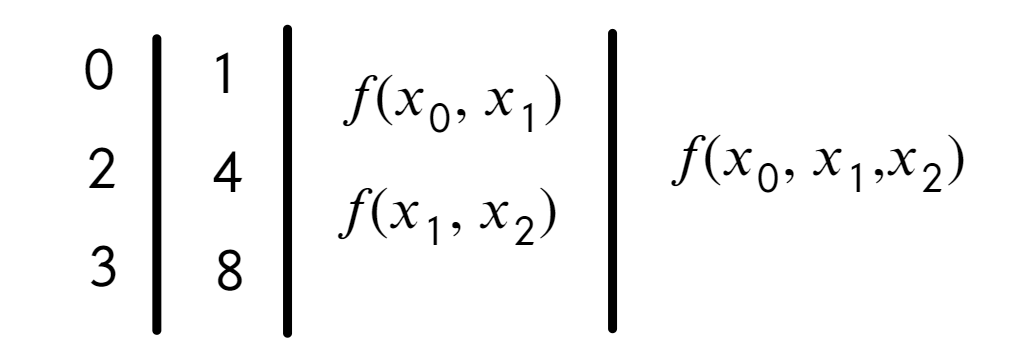
\includegraphics[scale=0.25]{img4}
	$$	
	По формуле (2) вычисляем значения для третьего столбца:
	$$f(x_0, x_1) = \dfrac{f(x_1) - f(x_0)}{x_1 - x_0} = \dfrac{4-1}{2-0} = \dfrac{3}{2},\quad f(x_1, x_2) = \dfrac{f(x_2) - f(x_1)}{x_2 - x_1} = \dfrac{8-4}{3-2} = 4.$$
	$$
	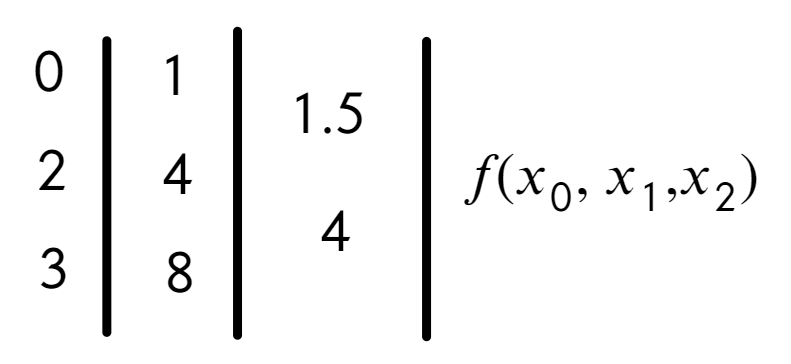
\includegraphics[scale=0.25]{img5}
	$$
	По формуле (3) вычисляем последнее неизвестное значение:
	$$f(x_0,x_1,x_2) = \dfrac{f(x_1, x_2) - f(x_0, x_1)}{x_2 - x_0} = \dfrac{4-1.5}{3-0} = \dfrac{5}{6}.$$
	Окончательно таблица имеет следующий вид, из которого нам понадобятся только выделенные значения:
	$$
	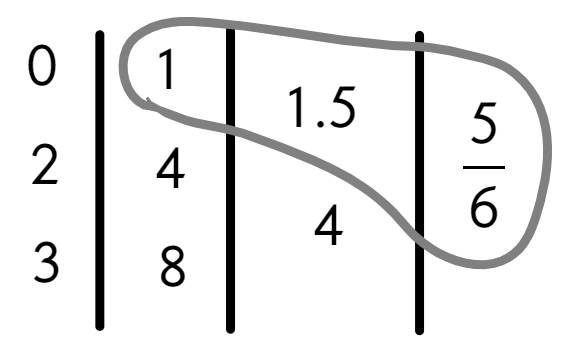
\includegraphics[scale=0.25]{img6}
	$$
	По формуле (1) строим интерполяционный многочлен, который в нашем случае имеет вид $$P_2(x) = f(x_0) + (x-x_0)\cdot f(x_0, x_1) + (x-x_0)(x-x_1)\cdot f(x_0,x_1,x_2).$$
	Подставляем все известные значения:
	$$P_2(x) = 1 + x\cdot \dfrac32 + x(x-2)\cdot \dfrac56 = \dfrac56x^2 - \dfrac16x + 1.$$
	Найдем значение в точке $x=0.5$:
	$$P_2(0.5) = \dfrac{5}{24} - \dfrac{1}{12} + 1 = \dfrac{27}{24}.$$
	Оценим остаток интерполирования, используя формулу (5):
	$$|r_n(x)| \leq \left|\omega_{n+1}(x) \dfrac{\underset{x\in[a,b]}{\max}|f^{(n+1)}(x)|}{(n+1)!}\right|.$$
	В нашем случае
	$$|r_2(x)| \leq \left|(x-x_0)(x-x_1)(x-x_2)| \dfrac{\underset{x\in[0,3]}{\max}|(2^x)^{(3)}(x)|}{3!}\right|.$$
	Так как $(2^^x)^{(n)} = \ln^n 2 2^x$, то $$\underset{x\in[0,3]}{\max}|2^x \cdot \ln^32|\leq (2\ln 2)^3.$$
	Тогда $$|r_2(x)|\leq \left|x(x-2)(x-3)\dfrac{(2\ln 2)^3}{6}\right|.$$
	Подставим точку, в которой мы проводили интерполирование, $x=0.5$:
	$$|r_2(0.5)|\leq \dfrac12\cdot \dfrac32\cdot\dfrac52\cdot\dfrac{(2\ln 2)^3}{6} = \dfrac52 \ln^32\approx 0.83256.$$
	Графически это можно представить как 
	\begin{center}\begin{tikzpicture}
			\begin{axis}[
				title = Function Interpolation,
				legend pos = north west,
				xlabel = {$x$},
				ylabel = {$y$},
				minor tick num = 2,
				xmin = -0.5,
				xmax = 3.5,
				grid = major,
				scatter/classes={%
					a={mark=o,draw=black}}
				]
				\legend{$2^x$, $P_2(x)$}
				\addplot[scatter,only marks,%
				scatter src=explicit symbolic]%
				table[meta=label] {
					x y label
					0 1 a
					2 4 a
					3 8 a
				};
				\addplot[orange] {5/6*x^2 - 1/6*x + 1};
			\end{axis}
	\end{tikzpicture}\end{center}

	\newpage
	\item 
	\hypertarget{t4}{}
	Для оценки погрешности интерполирования функции нам понадобятся следующие формулы:
	\begin{enumerate}
		\item остаток интерполирования при равноотстоящих узлах в начале таблицы \begin{eqnarray}
			r_k(x) =h^{k+1} \dfrac{t(t-1)\ldots (t-k)}{(k+1)!}f^{(k+1)}(\xi),\ \xi \in [x_0, x_0 + kh],\ t\in [0,1].
		\end{eqnarray}
		\item остаток интерполирования при равноотстоящих узлах в конце таблицы
		\begin{eqnarray}
			r_k(x) = h^{k+1}\dfrac{t(t+1)\ldots (t+k)}{(k+1)!}f^{(k+1)}(\xi),\ \xi \in [x_n, x_{n}-kh],\ t\in [-1,0].
		\end{eqnarray}
	\end{enumerate}
	Мы построим оценки для остатка интерполирования в начале таблицы и в конце таблицы и сравним полученные результаты.\\\\
	Сперва выпишем все данные, которые нам известны:\begin{itemize}
		\item интерполируемая функция $f(x) = \ln(x+2)$;
		\item сетка узлов на отрезке $[a,b] = [-1, 1]$;
		\item шаг $h = 0.1$;
		\item степень интерполяционного полинома $k=2$ (по условию квадратичная интерполяция).
	\end{itemize}
	Оценим остаток из формулы (1) при $k=2$:
	$$|r_2(x)| =\left|h^{3} \dfrac{t(t-1)(t-2)}{3!}f^{(3)}(\xi)\right|\leq h^{3}\left|\dfrac{t(t-1)(t-2)}{3!}\right|\cdot \underset{x\in[a,b]}{\max}|f^{(3)}(x)|,\ t\in [0,1].$$
	Оценим максимальное значение третьей производной на отрезке. Для этого вычислим третью производную от исходной функции $$f'(x) = \dfrac{1}{x+2},\quad f''(x) = -\dfrac{1}{(x+2)^2},\quad f'''(x) = \dfrac{2}{(x+2)^3}.$$
	Функция $\dfrac{2}{(x+2)^3}$ убывающая, следовательно, ее наибольшее значение в точке $x=-1$: $$\underset{x\in[-1,1]}{\max}|f^{(3)}(x)|= |f'''(-1)|= 2.$$
	Тогда, подставляя полученное значение и известное значение $h$ в формулу для оценки остатка, имеем $$|r_2(x)| \leq \dfrac{1}{3}\cdot10^{-3}\left|t(t-1)(t-2)\right|,\ t\in [0,1].$$
	Оценим значение выражения $\left|t(t-1)(t-2)\right|$. Для этого с помощью производной найдем точку максимума. Но сразу учтем, что $t\in [0,1]$ и при подстановке в это выражение точек $0$ и $1$ значение будет равно нулю, поэтому эти значения нас не интересуют. Рассмотрим функцию $$f(t) = t(t-1)(t-2) = t^3 - 3t^2 + 2t.$$
	Тогда $$f'(t) = 3t^2 - 6t + 2=0.$$
	Отсюда точки подозрительные на экстремумы $$t = 1\pm \dfrac{1}{\sqrt 3}.$$
	Но, так как $0<t<1$, то точка $1 + \dfrac{1}{\sqrt3}$ не подходит.
	Найдем значения в оставшейся точке
	$$f\left(1- \dfrac{1}{\sqrt 3}\right) = -\left(1- \dfrac{1}{\sqrt 3}\right)\cdot \dfrac{1}{\sqrt 3} \cdot \left(-1- \dfrac{1}{\sqrt 3}\right) = -\dfrac{2}{3\sqrt3}.$$
	Таким образом, $$\left|t(t-1)(t-2)\right|\leq \dfrac{2}{3\sqrt3}.$$
	Тогда мы можем вычислить оценку остатка интерполирования:
	$$|r_2(x)| \leq \dfrac{1}{3}\cdot \dfrac{2}{3\sqrt3}\cdot10^{-3}=\dfrac{2}{9\sqrt3}\cdot10^{-3}.$$
	Проделаем все то же самое для остатка интерполирования в конце таблицы из формулы (2): $$|r_2(x)| \leq \dfrac{1}{3}\cdot10^{-3}\left|t(t+1)(t+2)\right|,\ t\in [-1,0].$$
	То есть, нужно лишь оценить значение множителя с $t$. Снова точки $-1$, $0$ не рассматриваем. Рассмотрим функцию $$f(t) = t(t+1)(t+2) = t^3 + 3t^2 + 2t.$$
	Тогда $$f'(t) = 3t^2 + 6t + 2.$$
	Отсюда $$t = -1 \pm \dfrac{1}{\sqrt3}.$$
	Точка $-1 - \dfrac{1}{\sqrt3}$ не подходит. Вычислим значение в оставшейся точке: $$f\left(-1 + \dfrac{1}{\sqrt3}\right) = \left(-1 + \dfrac{1}{\sqrt3}\right)\cdot \dfrac{1}{\sqrt3}\cdot \left(1 + \dfrac{1}{\sqrt3}\right) = -\dfrac{2}{9\sqrt3}\cdot10^{-3}.$$
	То есть значение оценки остатка интерполирования будет таким же, что и в предыдущем случае.
	
	\newpage
	\item 
	\hypertarget{t5}{}
	Пусть функция $f(x)$ задана таблично в $n$ узлах $x_i$, которые являются равноотстоящими, то есть $$x_i = x_0 + ih,\ h>0,\quad i = 0,1,\ldots,n.$$
	Тогда интерполяционный многочлен будет иметь степень $n$.\\\\
	Интерполяционный многочлен Лагранжа записывается в общем виде \begin{eqnarray}
		P_n(x) = \sum_{k=0}^{n}l_k(x) f(x_k),\quad l_k(x) = \dfrac{\prod\limits_{j=0, j\ne k}^n (x-x_j)}{\prod\limits_{j=0, j\ne k}^n (x_k-x_j)}.
	\end{eqnarray}
	Тогда, поскольку узлы равноотстоящие, имеем \begin{itemize}
		\item $x - x_j = x - x_0 - jh$;
		\item $x_k - x_j = x_0 - kh - x_0 + jh = h(k-j)$.
	\end{itemize}
	Отсюда $$l_k(x) = \dfrac{\prod\limits_{j=0, j\ne k}^n (x - x_0 - jh)}{\prod\limits_{j=0, j\ne k}^n h(k-j)} = \dfrac{1}{h^n}\cdot \dfrac{\prod\limits_{j=0, j\ne k}^n (x - x_0 - jh)}{\prod\limits_{j=0, j\ne k}^n (k-j)}.$$
	Введем замену $t = \dfrac{x-x_0}{h}$.
	Отсюда \begin{multline*}
		l_k(x) = l_k(x_0 + th) = \dfrac{1}{h^n}\cdot \dfrac{\prod\limits_{j=0, j\ne k}^n (th - jh)}{\prod\limits_{j=0, j\ne k}^n (k-j)}=\prod\limits_{j=0, j\ne k}^n\dfrac{(t - j)}{(k-j)}=\\=\dfrac{t(t-1)\ldots (t-n)}{t-k}\cdot \dfrac{(-1)^{n-k}}{k!(n-k)!} = (-1)^{n-k} C^k_n\dfrac{1}{t-k}\cdot \dfrac{t(t-1)\ldots (t-n)}{n!}.
	\end{multline*}
	Подставим это в выражение (1), тогда $$P_n(x) = (-1)^n\dfrac{t(t-1)\ldots (t-n)}{n!}\sum_{k=0}^{n}(-1)^{-k}C^k_n\dfrac{1}{t-k}f(x_k).$$
	Недостатком данной формулы является факториальная сложность числителя и знаменателя, что делает вычисления достаточно трудоемкими. Поэтому при равноотстоящих узлах принято использовать интерполяционный многочлен в форме Ньютона.
	
	\newpage
	\item 
	\hypertarget{t6}{}
	Для решения данной задачи потребуются следующие формулы:
	\begin{enumerate}
		\item пусть функция $f(x)\in C^{n+1}[a,b]$ и для нее выполняется неравенство $$|f^{(n+1)}(x)|\leq M, \quad x\in [a,b],$$
		тогда погрешность интерполирования может быть оценена сверху следующим образом
		\begin{eqnarray}
			|r_n(x)| \leq \dfrac{M}{(n+1)!}\cdot \dfrac{(b-a)^{n+1}}{2^{2n+1}}.
		\end{eqnarray}
		\item значения узлов при оптимальном распределении на отрезке $[a,b]$
		\begin{eqnarray}
			x_k = \dfrac{a+b}{2} + \dfrac{b-a}{2}\cos \dfrac{(2k+1)\pi}{2(n+1)},\ k=\overline{0,n}.
		\end{eqnarray}
	\end{enumerate}
	Для отыскания степени $n$ многочлена интерполирования, будем решать неравенство $$|r_n(x)| \leq \dfrac{M}{(n+1)!}\cdot \dfrac{(b-a)^{n+1}}{2^{2n+1}}\leq \epsilon.$$
	Из-за того, что $n$ фигурирует и в качестве факториального значения, и в качестве степени, то решать уравнение придется подбором.\\\\
	Пусть $n=2$, тогда 
	$$|r_2(x)| \leq \dfrac{M}{3!}\cdot \dfrac{(5-2)^{3}}{2^{5}}\leq 10^{-5},\quad |f^{(3)}(x)|\leq M,\quad x\in [2,5]$$
	Оценим значение третьей производной от исходной функции:
	$$f'(x) = -2\sin 2x,\quad f''(x) =-4\cos2x ,\quad f'''(x) = 8\cos2x.$$
	Сделаем грубую оценку производной: $$|f'''(x)| = |8\cos2x| \leq 8 = M,\quad x\in [2;5].$$
	Тогда проверим, верное ли равенство:
	$$\dfrac{8}{6}\cdot \dfrac{27}{32}\leq 10^{-5}.$$
	Очевидно равенство не выполняется.\\\\
	Пусть $n=3$:
	$$|r_3(x)| \leq \dfrac{M}{4!}\cdot \dfrac{(5-2)^{4}}{2^{7}}\leq 10^{-5},\quad |f^{(4)}(x)|\leq M,\quad x\in [2,5]$$
	$$|f^{(4)}(x)| = |-16\sin2x| \leq 16 = M,\quad x\in [2;5].$$
	$$\dfrac{16}{24}\cdot \dfrac{81}{128}\leq 10^{-5}.$$
	Равенство не выполняется.
	\\\\
	Далее избежим оценки производной, считая, что $$|f^{(n+1)}(x)|\leq 2^{n+1}.$$
	Тогда $$|r_n(x)| \leq \dfrac{2^{n+1}}{(n+1)!}\cdot \dfrac{3^{n+1}}{2^{2n+1}} = \dfrac{1}{(n+1)!}\cdot \dfrac{3^{n+1}}{2^{n}}\leq \epsilon.$$
	И так далее подставляем $n=4,5,...,9$. При $n=11$ имеем $$|r_{10}(x)| \leq \dfrac{1}{11!}\cdot \dfrac{3^{11}}{2^{10}}\approx 4.33\cdot 10^{-6}.$$
	Таким образом, минимальная степень интерполяционного многочлена равна $10$.\\\\
	Укажем при этом распределение узлов по формуле (2):
	$$	x_k = \dfrac{7}{2} + \dfrac{3}{2}\cos \dfrac{(2k+1)\pi}{22},\ k=\overline{0,11}.$$
	
	\newpage
	\item 
	\hypertarget{t7}{}
	Для решения данной задачи потребуются следующие формулы:
	\begin{enumerate}
		\item остаток интерполирования при интерполировании с кратными узлами 
		\begin{eqnarray}
			r_n(x) = \Omega(x) \dfrac{f^{(n+1)}(\xi)}{(n+1)!},\quad \Omega (x) = (x-x_0)^{\alpha_0}\ldots (x-x_m)^{\alpha_m},\ \xi \in [a,b].
		\end{eqnarray}
		\item представление многочлена Эрмита через разделенные разности
		\begin{multline}
			P_n(x) = f(x_0) + (x-x_0)f(x_0, x_0) + \ldots + (x-x_0)^{\alpha_0-1}f(x_0,\ldots, x_0) + \\ + (x-x_0)^{\alpha_0}f(x_0,\ldots, x_0; x_1)+ (x-x_0)^{\alpha_0}(x-x_1)f(x_0,\ldots, x_0; x_1, x_1) +\ldots +\\+ \ldots + (x-x_0)^{\alpha_0}(x-x_1)^{\alpha_1-1} f(x_0,\ldots, x_0; x_1,\ldots, x_1) + \ldots+ \\\ +\ldots + (x-x_0)^{\alpha_0}(x-x_1)^{\alpha_1}\ldots(x-x_m)^{\alpha-1}f(x_0,\ldots x_0; x_1,\ldots, x_1; \ldots; x_{m},\ldots, x_{m}).
		\end{multline}
		\item для построения таблицы разделенных разностей, необходимо учитывать соотношение 
		\begin{eqnarray}
			f(\underbrace{x_0,\ldots, x_0}_{j+1}) = \dfrac{f^{(j)}(x_0)}{j!}
		\end{eqnarray}
		\item аппарат разделенных разностей:
		\begin{itemize}
			\item \textbf{разделенная разность нулевого порядка для функции $f(x)$} совпадают со значениями функции $f(x_i)$ в узлах интерполирования;
			\item \textbf{разделенная разность первого порядка} есть \begin{eqnarray}
				f(x_i, x_j) = \dfrac{f(x_j) - f(x_i)}{x_j - x_i}.
			\end{eqnarray}
			\item \textbf{разделенная разность второго порядка} \begin{eqnarray}
				f(x_i, x_j, x_k) = \dfrac{f(x_j, x_k) - f(x_i, x_j)}{x_k - x_i}.
			\end{eqnarray}
			\item \textbf{разделенная разность $(k+1)$-ого порядка} \begin{eqnarray}
				f(x_0, \ldots, x_{k+1}) = \dfrac{f(x_1,\ldots, x_{k+1}) - f(x_0,\ldots, x_k)}{x_{k+1} - x_0}.
			\end{eqnarray}
		\end{itemize}
		\item таблица разделенных разностей
		$$
		\includegraphics[scale=0.35]{"img9"}
		$$
	\end{enumerate}
	Алгоритм решения задачи следующий: составляем таблицу разделенных разностей, записываем интерполяционный многочлен, вычисляем значение в нужной точке, оцениваем остаток интерполирования в этой точке.\\\\
	Для начала рассчитаем входные данные:
	$$f(0) = 0,\quad f'(0) = 0,\quad f''(0) = 0,\quad f(1) = 1,\quad f'(1) = 6.$$
	Далее составляем таблицу конечных разностей, которая в нашем случае примет вид 
	$$
	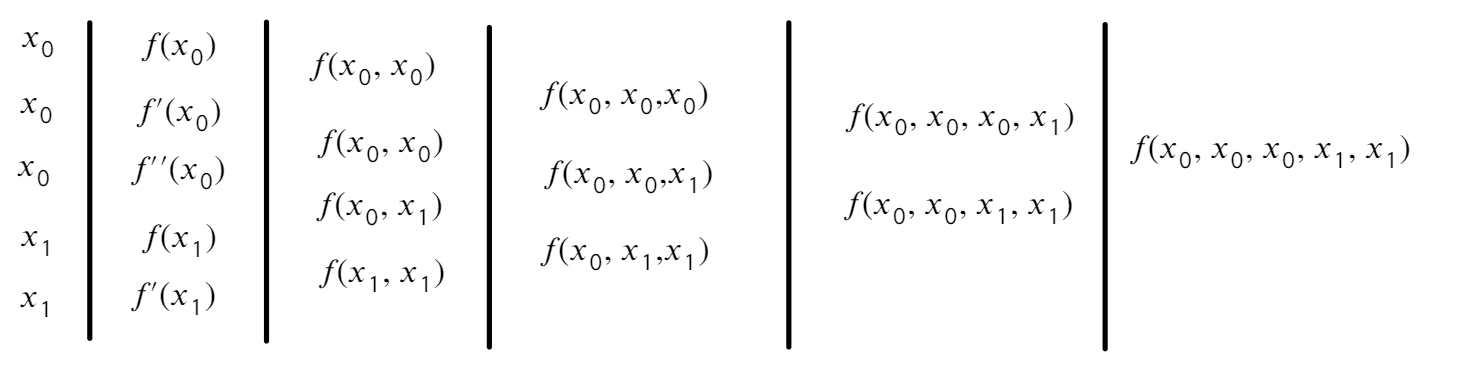
\includegraphics[scale=0.45]{img7}
	$$
	Заполним первые два столбца известными нам значениями:
	$$
	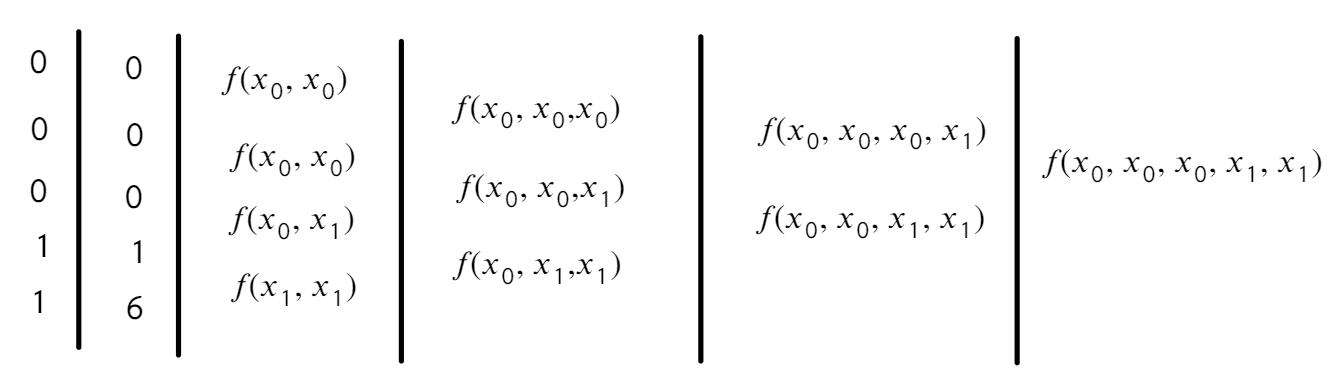
\includegraphics[scale=0.45]{img8}
	$$
	По формуле (3) $$f(x_0, x_0) = \dfrac{f'(x_0)}{1!} = 0,\quad f(x_1, x_1) = \dfrac{f'(x_1)}{1!} = 6.$$
	По формуле (4) $$f(x_0, x_1) = \dfrac{f(x_1) - f(x_0)}{x_1 - x_0} = 1.$$
	$$
	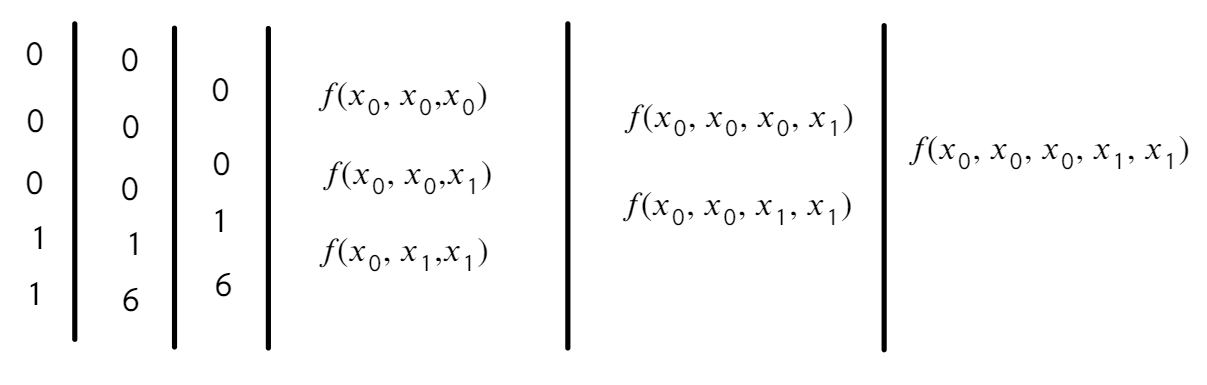
\includegraphics[scale=0.45]{img9}
	$$
	По формуле (3) $$f(x_0, x_0, x_0) = \dfrac{f'(x_0)}{2!} = 0.$$
	По формуле (5) $$f(x_0, x_0, x_1) = \dfrac{f(x_0,x_1) - f(x_0, x_0)}{x_1 - x_0} = 1,\quad f(x_0, x_1, x_1) = \dfrac{f(x_1,x_1) - f(x_0, x_1)}{x_1 - x_0} = 5.$$
	Далее аналогично по формуле (6)
	$$f(x_0, x_0, x_0, x_1) = \dfrac{f(x_0, x_0, x_1) - f(x_0, x_0, x_0)}{x_1 - x_0} = 1,$$ $$f(x_0, x_0, x_1, x_1) = \dfrac{f(x_0, x_1, x_1) - f(x_0, x_0, x_1)}{x_1 - x_0} = 4.$$
	И в итоге $$f(x_0,x_0,x_0,x_1,x_1) = \dfrac{f(x_0, x_0, x_1, x_1) -f(x_0, x_0, x_0, x_1) }{x_1 - x_0} = 3.$$
	Тогда таблица принимает окончательный вид
	$$
	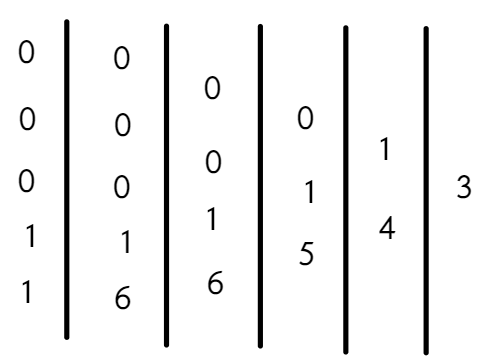
\includegraphics[scale=0.45]{img10}
	$$
	Из этой таблицы нам нужны лишь значения
	$$
	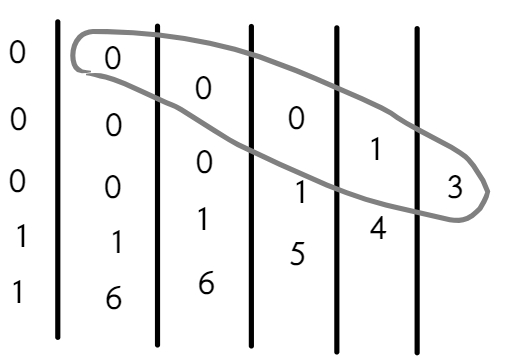
\includegraphics[scale=0.45]{img11}
	$$
	Далее по формуле (2) запишем сначала интерполяционный многочлен в общем виде для нашего случая (5 узлов $\Rightarrow$ 4 степень многочлена)
	\begin{multline*}
		P_4(x) = f(x_0) + (x-x_0)f(x_0, x_0) + (x-x_0)^2f(x_0, x_0,x_0)+\\+ (x-x_0)^3f(x_0, x_0,x_0, x_1) + (x-x_0)^3(x-x_1)f(x_0, x_0,x_0, x_1, x_1).
	\end{multline*}
	Подставляем все известные нам значения и получаем
	$$P_4(x) = 0 + x\cdot 0 + x^2\cdot 0 + x^3\cdot 1 + x^3(x_1)\cdot 3 = 3x^4 - 2x^3.$$
	Можно, подставив известные точки и их значения, убедиться в том, что многочлен был построен правильно. \\\\
	Вычислим значение в точке $x=0.5$:
	$$P_4(0.5) = \dfrac{3}{16} - \dfrac{2}{8} = -\dfrac{1}{16}.$$
	Оценим остаток по формуле (1). Для начала запишем его в общем виде для нашего случая:
	$$r_4(x) = (x-x_0)^3 ( x-x_1)^2\cdot \dfrac{f^{(5)}(\xi)}{5!},\quad \xi \in [0,1].$$
	Нам неизвестно значение $f^{(5)}(\xi)$. Оценим его сверху:
	$$f^{(5)}(x) = (x^6)^{(5)} = 720 x\Rightarrow |f^{(5)}(x)| \leq 720 \quad x\in [0,1].$$
	Тогда оценка для остатка примет вид
	$$|r_4(x)|\leq \left|x^3 ( x-1)^2\cdot \dfrac{720}{120}\right| = 6\left|x^3 ( x-1)^2\right|.$$
	Отсюда погрешность вычисленного значения в точке $x=0.5$ составляет $$|r_4(0.5)|\leq 6\left|\dfrac{1}{2^3} \cdot\dfrac{1}{2^2}\right| = \dfrac{3}{16}.$$
	
	\newpage
	\item 
	\hypertarget{t8}{}
	Многочлены Чебышева задаются формулой $$T_n(x) = \cos (n\arccos x).$$
	Чтобы функции являлись решениями дифференциального уравнения, они должны при подстановке в уравнение давать верное равенство. \\\\
	Вычислим первую и вторую производные от многочленов Чебышева:
	$$T'_n(x) = \dfrac{n \sin (n\arccos x)}{\sqrt{1-x^2}};$$
	$$T''_n(x) = \dfrac{n^2\cos (n\arccos x) \cdot (-\frac{1}{\sqrt{1-x^2}})\cdot \sqrt{1-x^2} + \frac{2x}{2\sqrt{1-x^2}} \cdot n \sin (n\arccos x)}{1-x^2}.$$
	Подставим найденные производные в данное по условию дифференциальное уравнение:
	$$(1-x^2)\cdot \dfrac{-n^2\cos (n\arccos x) + \frac{x}{\sqrt{1-x^2}} \cdot n \sin (n\arccos x)}{1-x^2} -x\cdot \dfrac{n \sin (n\arccos x)}{\sqrt{1-x^2}} + n^2 \cos(n\arccos x) = 0.$$
	Равенство выполняется, следовательно, многочлены Чебышева являются решениями данного дифференциального уравнения.
	
	\newpage
	\item 
	\hypertarget{t9}{}
	Для решения данной задачи потребуются следующие формулы:
	\begin{enumerate}
		\item многочлены Чебышева $T_n(x)$, $n\geq 0$ определенные на отрезке $[-1,1]$, задающиеся соотношениями 
		\begin{eqnarray}
			T_0(x)=1,\ T_1(x) = x,\ T_{n+1}(x) = 2xT_n(x) - T_{n-1}(x),\quad n=1,2,\ldots.
		\end{eqnarray}
		\item вид многочленов Чебышева на отрезке $[a,b]$ 
		\begin{eqnarray}
			\hat T_{n+1}(x) = \dfrac{(b-a)^{n+1}}{2^{2n+1}} T_{n+1}\Big(\dfrac{2x - (b+a)}{b-a}\Big),\ x\in [a,b].
		\end{eqnarray}
	\end{enumerate}
	Известно также, что многочлены Чебышева являются наименее отклоняющимися от нуля многочленами степени $n$ на отрезке $[-1,1]$ среди всех многочленов степени $n$ заданных на этом отрезке.\\\\
	Таким образом, нам необходимо, используя формулы (1) и (2), задать многочлен Чебышева на отрезке $[1,5]$, после чего привести его к нужному виду (чтобы коэффициент при $x^2$ был равен 3).\\\\
	Из соотношений (1) выясним, какой вид имеет многочлен Чебышева 3-ей степени:
	$$T_2(x) = 2x^2 - 1,\quad T_3(x) = 4x^2 - 2x - x = 4x^3 - 3x.$$
	Теперь в формулу (2) подставим отрезок $[a,b] = [1,5]$:
	$$T_{n+1}(x) = \dfrac{4^{n+1}}{2^{2n + 1}}\cdot T_{n+1}\left(\dfrac{2x - 6}{4}\right).$$
	Подставим в формулу (2) $n=2$:
	$$\hat T_{3}(x) = \dfrac{4^{3}}{2^{5}}\cdot T_{3}\left(\dfrac{2x - 6}{4}\right)=2T_{3}\left(\dfrac{2x - 6}{4}\right).$$
	Найдем $T_{3}\left(\dfrac{2x - 6}{4}\right)$:
	\begin{multline*}
		T_{3}\left(\dfrac{2x - 6}{4}\right) = 4\left(\dfrac{x}{2} - \dfrac{3}{2}\right)^3 - 3\left(\dfrac{x}{2} - \dfrac{3}{2}\right) = 4\left(\dfrac{x^3}{8} - \dfrac{9x^2}{8} + \dfrac{27x}{8}-\dfrac{27}{8}\right) - \dfrac{3x}{2} + \dfrac{9}{2} =\\ = \dfrac{x^3}{2} - \dfrac{9x^2}{2} + \dfrac{24x}{2} - \dfrac{18}{2}.
	\end{multline*}
	Тогда $$\hat T_3(x) = x^3 - 9x^2 + 24x - 18,\quad x\in [1,5].$$
	Мы получили многочлен наименее отклоняющийся от нуля на отрезке $[1,5]$. Чтобы он удовлетворял указанному виду, домножим его на $-\dfrac13$:
	$$P_3(x) = -\dfrac13 x^3 + 3x^2 - 8x + 6.$$
	
	\newpage
	\item 
	\hypertarget{t10}{}
	В гильбертовом пространстве система функций $\{\varphi_i\}$ ортогональна, если $(\varphi_i, \varphi_j) =0$ $\forall i\ne j$. \\\\
	Возьмем гильбертово пространство $L_2[-1,1]$ с весом $p(x) = \dfrac{1}{\sqrt{1-x^2}}$. В данном случае $$(\varphi_i, \varphi_j) = \int\limits_{-1}^1 p(x)\varphi_i(x)\varphi_j(x) dx.$$
	Также, поскольку система функций является системой многочленов Чебышева, то $$\varphi_k(x) = T_k(x) = \cos (k\arccos x).$$
	Найдем скалярное произведение двух производных функций из системы многочленов Чебышева:
	\begin{multline*}
		(T_i(x), T_j(x)) = \int\limits_{-1}^1 \dfrac{\cos (i\arccos x)\cos(j \arccos x)}{\sqrt{1-x^2}} dx = \left[\begin{matrix}
			\arccos x = t, & x = \cos t\\
			x=-1 \to t=\pi, & x=1 \to t = 0\\
			dx = -\sin t dt
		\end{matrix}\right] =\\ = \int\limits_{0}^\pi \dfrac{\cos (it)\cos(j t)}{\sqrt{1-\cos t^2}}\sin t\ dt = \int\limits_{0}^\pi \cos (it)\cos(j t) dt = \dfrac12\int\limits_{0}^\pi \cos ((i+j)t)+\cos((i-j) t) dt=\\= \dfrac{1}{2(i+j)}\sin ((i+j)t)\Big|_0^\pi + \dfrac{1}{2(i-j)}\sin ((i-j)t)\Big|_0^\pi = 0,\quad i \ne j.
	\end{multline*}
	Таким образом, система многочленов Чебышева при заданных условиях является ортогональной.
	
	\newpage
	\item \hypertarget{t11}{}
	Для решения данной задачи нам понадобятся следующие формулы ($N$ -- количество узлов):\begin{enumerate}
		\item расстояние между $i$-ым и $(i-1)$-ым узлами \begin{eqnarray}
			h_i=x_i - x_{i-1},\qquad i=\overline{1,N}\label{1}
		\end{eqnarray}
		\item формула кубического сплайна\begin{multline}
			S_3(x) = M_{i-1}\dfrac{(x_i - x)^3}{6h_i} + M_{i}\dfrac{(x-x_{i-1})^3}{6h_i} + \left(f_i - M_i\dfrac{h_i^2}{6}\right)\dfrac{x-x_{i-1}}{h_i} +\\+ \left(f_{i-1} - M_{i-1}\dfrac{h_i^2}{6}\right)\dfrac{(x_i - x)}{h_i},\quad x\in [x_{i-1}, x_i],\ i = \overline{1,N}
		\end{multline}
		\item формулы для коэффициентов кубического сплайна
		\begin{multline}
			\dfrac{h_i}{6}M_{i-1} + \dfrac{h_i + h_{i+1}}{3}M_i + \dfrac{h_{i+1}}{6}M_{i+1} = \dfrac{f_{i+1} - f_i}{h_{i+1}} - \dfrac{f_i - f_{i-1}}{h_i},\quad i = \overline {1,N-1}
		\end{multline}
		\item естественные граничные условия для коэффициентов (так как не заданы значения производных) \begin{eqnarray}
			M_0 = 0,\quad M_N = 0.
		\end{eqnarray}
	\end{enumerate}
	Сначала по формуле (1) найдем расстояния между узлами:
	$$\begin{matrix}
		h_1 = x_1 - x_0 = 1,\\
		h_2 = x_2 - x_1 = 1,\\
		h_3 = x_3 - x_2 = 2.
	\end{matrix}$$
	Теперь составим по формулам (3) и (4) СЛАУ для коэффициентов кубического сплайна:
	$$\begin{cases}
		M_0 = 0,\\
		\dfrac{h_1}{6}M_{0} + \dfrac{h_1 + h_{2}}{3}M_1 + \dfrac{h_{2}}{6}M_{2} = \dfrac{f_{2} - f_1}{h_{2}} - \dfrac{f_1 - f_{0}}{h_1},\\
		\dfrac{h_2}{6}M_{1} + \dfrac{h_2 + h_{3}}{3}M_2 + \dfrac{h_{3}}{6}M_{3} = \dfrac{f_{3} - f_2}{h_{3}} - \dfrac{f_2 - f_{1}}{h_2},\\
		M_3 = 0.
	\end{cases}$$
	Подставим в эту систему значения ($h_i$ нам известны, $M_1 = M_3 = 0$):
	$$\begin{cases}
		M_0 = 0,\\
		\dfrac{1 + 1}{3}M_1 + \dfrac{2}{6}M_{2} = \dfrac{5 - 3}{1} - \dfrac{3 - 2}{1},\\\\
		\dfrac{1}{6}M_{1} + \dfrac{1+2}{3}M_2 = \dfrac{10 - 5}{2} - \dfrac{5 - 3}{1},\\
		M_3=0.
	\end{cases}
	\Rightarrow 
	\begin{cases}
		M_0 = 0,\\
		\dfrac{2}{3}M_1 + \dfrac{1}{3}M_{2} = 1,\\\\
		\dfrac{1}{6}M_{1} + M_2 = \dfrac12,\\
		M_3=0.
	\end{cases}$$
	Найдем методом Гаусса коэффициенты $M_1, M_2$:
	$$
	\begin{pmatrix}
		\frac23&\frac16&\vline&1\\
		\frac16&1&\vline&\frac12
	\end{pmatrix}
	\sim
	\begin{pmatrix}
		1&\frac14&\vline&\frac32\\
		0&\frac{23}{4}&\vline&\frac32
	\end{pmatrix}
	\sim 
	\begin{pmatrix}
		1&\frac14&\vline&\frac32\\
		0&1&\vline&\frac{6}{23}
	\end{pmatrix}
	\sim
	\begin{pmatrix}
		1&0&\vline&\frac{33}{23}\\
		0&1&\vline&\frac{6}{23}
	\end{pmatrix}$$
	То есть $$M_0 = 0,\quad M_1 = \dfrac{33}{23},\quad M_2 = \dfrac{6}{23},\quad M_3 = 0.$$
	У нас есть все необходимые значения для того, чтобы построить кубический сплайн, кроме $x_i$, $x_{i-1}$. По условию необходимо вычислить значение в точке $x=3$, она находится между узлами $x_2 = 2$ и $x_3 = 4$. Тогда кубический сплайн по формуле (2) мы будем строить на узлах $x_1, x_2$.\\\\
	В нашем случае формула (2) примет вид 
	\begin{multline*}
		S_3(x) = M_2\dfrac{(x_3 - x)^3}{6h_3} + M_{3}\dfrac{(x-x_2)^3}{6h_3} + \left(f_3 - M_3\dfrac{h_3^2}{6}\right)\dfrac{x-x_2}{h_3} +\\+ \left(f_2 - M_2\dfrac{h_3^2}{6}\right)\dfrac{(x_3 - x)}{h_3},\quad x\in [x_2, x_3].
	\end{multline*}
	Подставляем все известные нам значения:
	$$
	S_3(x) = \dfrac{6}{23}\cdot\dfrac{(4 - x)^3}{12} + 10\cdot\dfrac{x-2}{2} + \left(5 - \dfrac{6}{23}\cdot\dfrac{4}{6}\right)\dfrac{(4 - x)}{2},\quad x\in [2, 4].
	$$
	Сделаем некоторые преобразования для упрощения формулы
	$$
	S_3(x) = \dfrac{(4 - x)^3}{46} + \dfrac{119x}{46}-\dfrac{8}{23},\quad x\in [2, 4].
	$$
	Найдем значение в точке $x=3$:
	$$
	S_3(3) = \dfrac{1}{46} + \dfrac{357}{46} - \dfrac{8}{23} = \dfrac{171}{23}.
	$$
	\newpage
	\item 
	\hypertarget{t12}{}
	Для решения данной задачи нам понадобятся следующие формулы ($N$ -- количество узлов):\begin{enumerate}
		\item расстояние между $i$-ым и $(i-1)$-ым узлами \begin{eqnarray}
			h_i=x_i - x_{i-1},\qquad i=\overline{1,N}\label{1}
		\end{eqnarray}
		\item формула кубического сплайна\begin{multline}
			S_3(x) = M_{i-1}\dfrac{(x_i - x)^3}{6h_i} + M_{i}\dfrac{(x-x_{i-1})^3}{6h_i} + \left(f_i - M_i\dfrac{h_i^2}{6}\right)\dfrac{x-x_{i-1}}{h_i} +\\+ \left(f_{i-1} - M_{i-1}\dfrac{h_i^2}{6}\right)\dfrac{(x_i - x)}{h_i},\quad x\in [x_{i-1}, x_i],\ i = \overline{1,N}
		\end{multline}
		\item формулы для коэффициентов кубического сплайна
		\begin{multline}
			\dfrac{h_i}{6}M_{i-1} + \dfrac{h_i + h_{i+1}}{3}M_i + \dfrac{h_{i+1}}{6}M_{i+1} = \dfrac{f_{i+1} - f_i}{h_{i+1}} - \dfrac{f_i - f_{i-1}}{h_i},\quad i = \overline {1,N-1}
		\end{multline}
		\item граничные условия для коэффициентов \begin{eqnarray}
			M_0 = f''(a),\quad M_N = f''(b).
		\end{eqnarray}
	\end{enumerate}
	Сначала по формуле (1) найдем расстояния между узлами:
	$$\begin{matrix}
		h_1 = x_1 - x_0 = 1\\
		h_2 = x_2 - x_1 = 3.
	\end{matrix}$$
	Теперь составим по формулам (3) и (4) СЛАУ для коэффициентов кубического сплайна:
	$$\begin{cases}
		M_0 = f''(a),\\
		\dfrac{h_1}{6}M_{0} + \dfrac{h_1 + h_{2}}{3}M_1 + \dfrac{h_{2}}{6}M_{2} = \dfrac{f_{2} - f_1}{h_{2}} - \dfrac{f_1 - f_{0}}{h_1},\\
		M_2 = f''(b).
	\end{cases}$$
	Подставим в эту систему значения ($h_i$ нам известны, $f_i$ и $f''(a)$, $f''(b)$ берем из заданной таблицы):
	$$\begin{cases}
		M_0 = 3,\\
		\dfrac{1}{6}M_{0} + \dfrac{1+3}{3}M_1 + \dfrac{3}{6}M_{2} = \dfrac{9 -1}{3} - \dfrac{1 - 0}{1},\\
		M_2=5.
	\end{cases}
	\Rightarrow 
	\begin{cases}
		M_0 = 3,\\
		\dfrac{1}{6}M_{0} + \dfrac43M_1 + \dfrac{1}{2}M_{2} = \dfrac53,\\
		M_{2}=5.
	\end{cases}$$
	Найдем решение методом Гаусса 
	$$\begin{pmatrix}
		1&0&0&\vline&3\\
		1&8&3&\vline&10\\
		0&0&1&\vline&5
	\end{pmatrix}
	\sim 
	\begin{pmatrix}
		1&0&0&\vline&3\\
		0&8&0&\vline&-8\\
		0&0&1&\vline&5
	\end{pmatrix}
	\sim
	\begin{pmatrix}
		1&0&0&\vline&3\\
		0&1&0&\vline&-1\\
		0&0&1&\vline&5
	\end{pmatrix}$$
	То есть $$M_0 = 3,\quad M_1 = -1,\quad M_2 = 5.$$
	У нас есть все необходимые значения для того, чтобы построить кубический сплайн, кроме $x_i$, $x_{i-1}$. По условию необходимо вычислить значение в точке $x=3$, она находится между узлами $x_1 = 2$ и $x_2 = 5$. Тогда кубический сплайн по формуле (2) мы будем строить на узлах $x_1, x_2$.\\\\
	В нашем случае формула (2) примет вид \begin{multline*}
		S_3(x) = M_1\dfrac{(x_2 - x)^3}{6h_2} + M_{2}\dfrac{(x-x_1)^3}{6h_2} + \left(f_2 - M_2\dfrac{h_2^2}{6}\right)\dfrac{x-x_1}{h_2} +\\+ \left(f_1 - M_1\dfrac{h_2^2}{6}\right)\dfrac{(x_2 - x)}{h_2},\quad x\in [x_1, x_2].
	\end{multline*}
	Подставляем все известные нам значения:
	$$
	S_3(x) = -\dfrac{(5 - x)^3}{18} +5\cdot\dfrac{(x-2)^3}{18} + \left(9 -5\cdot\dfrac{9}{6}\right)\dfrac{x-2}{3} + \left(1 + \dfrac{9}{6}\right)\dfrac{(5 - x)}{3},\quad x\in [2, 5].
	$$
	Сделаем некоторые преобразования для упрощения формулы
	$$
	S_3(x) = \dfrac{5(x - 2)^3 - (5-x)^3}{18} + \dfrac{x-2}{2} + \dfrac{5(5 - x)}{6},\quad x\in [2, 5].
	$$
	Найдем значение в точке $x=3$:
	$$
	S_3(3) = \dfrac{5 - 8}{18} + \dfrac{1}{2} + \dfrac{5\cdot 2}{6} = 2.
	$$
	\newpage
	\item 
	\hypertarget{t13}{}
	Для решения данной задачи нам понадобятся следующие формулы ($N$ -- количество узлов):\begin{enumerate}
		\item расстояние между $i$-ым и $(i-1)$-ым узлами \begin{eqnarray}
			h_i=x_i - x_{i-1},\qquad i=\overline{1,N}\label{1}
		\end{eqnarray}
		\item формула кубического сплайна\begin{multline}
			S_3(x) = M_{i-1}\dfrac{(x_i - x)^3}{6h_i} + M_{i}\dfrac{(x-x_{i-1})^3}{6h_i} + \left(f_i - M_i\dfrac{h_i^2}{6}\right)\dfrac{x-x_{i-1}}{h_i} +\\+ \left(f_{i-1} - M_{i-1}\dfrac{h_i^2}{6}\right)\dfrac{(x_i - x)}{h_i},\quad x\in [x_{i-1}, x_i],\ i = \overline{1,N}
		\end{multline}
		\item формулы для коэффициентов кубического сплайна
		\begin{multline}
			\dfrac{h_i}{6}M_{i-1} + \dfrac{h_i + h_{i+1}}{3}M_i + \dfrac{h_{i+1}}{6}M_{i+1} = \dfrac{f_{i+1} - f_i}{h_{i+1}} - \dfrac{f_i - f_{i-1}}{h_i},\quad i = \overline {1,N-1}
		\end{multline}
		\item граничные условия для коэффициентов \begin{eqnarray}
			\begin{cases}
				2M_0 + M_1 = \dfrac{6}{h_1}\left(\dfrac{f_1-f_0}{h_1} - f'(a)\right),\\
				M_{N-1} + 2M_N = \dfrac{6}{h_N}\left(f'(b) - \dfrac{f_N-f_{N-1}}{h_N} \right).
			\end{cases}
		\end{eqnarray}
	\end{enumerate}
	Сначала по формуле (1) найдем расстояния между узлами:
	$$\begin{matrix}
		h_1 = x_1 - x_0 = 2\\
		h_2 = x_2 - x_1 = 1.
	\end{matrix}$$
	Теперь составим по формулам (3) и (4) СЛАУ для коэффициентов кубического сплайна:
	$$\begin{cases}
		2M_0 + M_1 =  \dfrac{6}{h_1}\left(\dfrac{f_1-f_0}{h_1} - f'(a)\right),\\
		\dfrac{h_1}{6}M_{0} + \dfrac{h_1 + h_{2}}{3}M_1 + \dfrac{h_{2}}{6}M_{2} = \dfrac{f_{2} - f_1}{h_{2}} - \dfrac{f_1 - f_{0}}{h_1},\\
		M_{1} + 2M_2 = \dfrac{6}{h_2}\left(f'(b) - \dfrac{f_2-f_{1}}{h_2} \right).
	\end{cases}$$
	Подставим в эту систему значения ($h_i$ нам известны, $f_i$ и $f'(a)$, $f'(b)$ берем из заданной таблицы):
	$$\begin{cases}
		2M_0 + M_1 =  \dfrac{6}{2}\left(\dfrac{5-1}{2} - 1\right),\\
		\dfrac{2}{6}M_{0} + \dfrac{2 +1}{3}M_1 + \dfrac{1}{6}M_{2} = \dfrac{7 -5}{1} - \dfrac{5 - 1}{2},\\
		M_{1} + 2M_2 = \dfrac{6}{1}\left(0 - \dfrac{7-5}{1} \right).
	\end{cases}
	\Rightarrow 
	\begin{cases}
		2M_0 + M_1 =  3,\\
		\dfrac{1}{3}M_{0} + M_1 + \dfrac{1}{6}M_{2} = 0,\\
		M_{1} + 2M_2 = -12.
	\end{cases}$$
	Найдем решение методом Гаусса 
	$$\begin{pmatrix}
		2&1&0&\vline&3\\
		2&6&1&\vline&0\\
		0&1&2&\vline&-12
	\end{pmatrix}
	\sim 
	\begin{pmatrix}
		1&\frac12&0&\vline&\frac32\\
		0&5&1&\vline&-3\\
		0&1&2&\vline&-12
	\end{pmatrix}
	\sim
	\begin{pmatrix}
		1&\frac12&0&\vline&\frac32\\
		0&1&2&\vline&-12\\
		0&0&-9&\vline&-57
	\end{pmatrix}
	\sim
	\begin{pmatrix}
		1&0&0&\vline&\frac76\\
		0&1&0&\vline&\frac{2}{3}\\
		0&0&1&\vline&-\frac{19}{3}
	\end{pmatrix}$$
	То есть $$M_0 = \dfrac76,\quad M_1 = \dfrac23,\quad M_2 = -\dfrac{19}{3}.$$
	У нас есть все необходимые значения для того, чтобы построить кубический сплайн, кроме $x_i$, $x_{i-1}$. По условию необходимо вычислить значение в точке $x=1$, она находится между узлами $x_0 = 0$ и $x_1 = 2$. Тогда кубический сплайн по формуле (2) мы будем строить на узлах $x_0, x_1$.\\\\
	В нашем случае формула (2) примет вид \begin{multline*}
		S_3(x) = M_0\dfrac{(x_1 - x)^3}{6h_1} + M_{1}\dfrac{(x-x_0)^3}{6h_1} + \left(f_1 - M_1\dfrac{h_1^2}{6}\right)\dfrac{x-x_0}{h_1} +\\+ \left(f_0 - M_0\dfrac{h_1^2}{6}\right)\dfrac{(x_1 - x)}{h_1},\quad x\in [x_0, x_1].
	\end{multline*}
	Подставляем все известные нам значения:
	$$
	S_3(x) = \dfrac76\dfrac{(2 - x)^3}{12} + \dfrac23\cdot\dfrac{x^3}{12} + \left(5 - \dfrac23\cdot\dfrac{4}{6}\right)\dfrac{x}{2} + \left(1 - \dfrac76\cdot\dfrac{4}{6}\right)\dfrac{(2 - x)}{2},\quad x\in [0, 2].
	$$
	Сделаем некоторые преобразования для упрощения формулы
	$$
	S_3(x) = \dfrac{7(2 - x)^3}{72} + \dfrac{x^3}{18} + \dfrac{22x}{9} + \dfrac{(2 - x)}{9},\quad x\in [0, 2].
	$$
	Найдем значение в точке $x=1$:
	$$
	S_3(1) = \dfrac{7}{72} + \dfrac{1}{18} + \dfrac{22}{9} + \dfrac{1}{9} = \dfrac{195}{72}.
	$$
	\end{enumerate}
\end{document} 